\chapter{Kinematics}
\minitoc
\bigskip

The robot kinematic model along with encoder measurements make possible the computation of poses and spatial velocities \cite{featherstone2014rigid} (aka. twists) 
of reference frames attached to the robot segments relative to the base or world frame. This kinesthesis capability is of paramount importance to control
multi-body systems for locomotion or other interactions with their environment. If we have information about stable contacts that the robot keeps with
its environment, it is possible to infer a relative motion measurement, which is commonly called leg-odometry.

We will shortly describe the formulation of the forward-kinematics algorithm, that enables to compute relative poses and spatial velocities between parts of the robot
and then show how this information can be used to define a leg-odometry factor to be added in the factor graph. The last section shows how forward-kinematics can also be used to leverage prior 
information about the height of the environment. 



\section{Forward kinematics}
\label{sec:forward_kinematics}
We first describe the forward-kinematics and differential kinematics algorithms by introducing notations commonly found in the legged robots literature.

The degrees of freedom (DoF) $n$ of a poly-articulated system is the minimal number of variables that completely describe his state given the base frame. 
For robots with rigid segments, the DoF of the robot is the sum of the DoFs of its joints (1 for linear and rotational joints, 3 for
ball joints, etc.).
The state of the joints (1 angle for rotational joints) can be stacked together in the vector of joint configurations 
$\qa \in \Reals^n$. For most simple joints, the joint configuration velocities are simply the time derivative $\dqa \in \Reals^n$\footnote{An exception is the ball joint where the 
state is defined as an element of $\SO(3)$, thus its velocity vector is defined as an angular velocity in $\Reals^3$.}. $\qa$ and $\dqa$ are typically obtained from
the joint encoder measurements.
Legged robots are not fixed to the ground so we add a so-called "free-flyer" FoF which represents the free pose of the base with respect to the world and is modeled as an 
unactuated joint of 6 DoF pertaining to the $\SE(3)$ group. Its velocities are therefore in the $\se(3)$  Lie algebra, isomorphic to $\Reals^6$. 

The whole-body state of the robot is defined by the robot configuration vector $\bfq=[\bfq_b,\qa]\in \SE(3) \times \Reals^n$, where 

\begin{equation}
    \bfq_b \triangleq \T{W}{B} =  
    \begin{pmatrix}
        \Rot{W}{B} & \posi{W}{B} \\
        \bf0_3\tr & 1
    \end{pmatrix}
\end{equation}
%
is the configuration of the base,
with $\posi{w}{b} \in \Reals^3$ and $\Rot{W}{B} \in \SO(3)$ are the position and orientation of the base with respect to the world.
$\qa \in \Reals^n$ is the configuration of the joints. $\bfq$ therefore belongs to a composite manifold $\cM_{\bfq} = \left<\SE(3), \Reals^n \right>$ and the configuration velocity vector belongs to its tangent space $\se(3)\times \Reals^n$ which is isomorphic to $\Reals^{6+n}$: $\bfv_q \in \Reals^{6+n}$. Those are concatenations
of the base state and joint configuration vectors:
%
\begin{equation}
    \bfq= [\bfq_b, \qa]\in \cM_{\bfq}\quad\quad,
    \quad\quad
    \bfv_q= [\prescript{b}{}{\mathbf{\nu}}_b,\dqa]  \in \Reals^{6+n}
    \label{eq:configuration}
\end{equation}
%
where $\prescript{b}{}{\mathbf{\nu}}_b$ is the twist of the base frame expressed in the base frame.
The computation of any segment pose of index $k$ relative to the world is obtained using the forward-kinematics (FK) algorithm:
%
\begin{equation}
    \T{W}{K} = \text{FK}_k(\bfq)
\end{equation}

The kinematic chains of most robots is can be represented as a tree whose root is the world frame, nodes are the joints to which are associated reference frames (including the base, which is considered as a $\SE(3)$ joint), and edges are solid segment placed between these nodes.
The forward-kinematics algorithm consists of a forward pass from the root of the tree $\T{W}{B}$ through the joints along the path to the leaf $\T{W}{K}$ that we wish to obtain. Let us denote by $i$ the index of each intermediate joint between the root and the leaf, the root (world) having index 0 and the base index 1, the forward-kinematics algorithm simply writes as a composition of successive transformations:

\begin{equation}
    \Tbar{0}{k} = \T{0}{1}(\bfq_b) \Tbar{1}{2'}
    \T{2'}{2}(q_2) \dots  \Tbar{k-1}{k'} \T{k'}{k}(q_k)
\end{equation}
%
where $\Tbar{i-1}{i'}$ designates the transformation between joint frames $i-1$ and $i$ when the joint configuration $q_i$ is at the identity value and is a constant. 
The $\T{i'}{i}(q_i)$ designate transformations caused by a non-zero joint value $q_i$, as reprsented in \figRef{fig:forward_kinematics}.

\begin{figure}
    \centering
    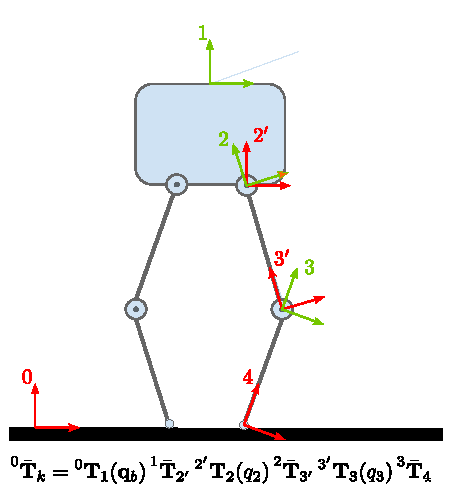
\includegraphics[width=0.5\textwidth]{figures/kinematic_tree_FK.pdf}
    \caption{Illustration of the Forward kinematics algorithm to get the transformation of the foot $4$ with respect to the world $0$.}
    \label{fig:forward_kinematics}
\end{figure}


It is also possible to obtain the pose relative to the base $\T{b}{k}$ by simply setting the base pose vector to be the identity pose $[0,0,0,~0,0,0,1]$.

% Differential FK is not used anywhere so...
% FK is a nonlinear function of the robot configuration. 
% To obtain the relative spatial velocity, we have to compute the Jacobian $\bfJ_k$ of FK with respect to the configuration.
% The differential forward-kinematics (DFK) is then simply:

% \begin{equation}
%     \prescript{w}{}{\mathbf{\nu}}_k = \bfJ_k \bfv_q    
% \end{equation}

Similarly, the spatial velocity relative to the base $\prescript{b}{}{\mathbf{\nu}}_k$ can be obtained by setting the base spatial velocity part of $\bfv_q$ to zero.
These algorithms are very fast to compute ($\approx 1\mu s)$ using modern dedicated libraries \cite{carpentier2019pinocchio}.

We will now see how FK can be used to derive leg-odometry for a quadruped robot.

\section{Leg odometry}
\label{sec:leg_odometry}
We will restrict ourselves to the case of point feet as the main platform on which we experimented is a quadruped robot.
Quadrupeds are usually equipped with non-articulated round feet whose contact with the ground is, in first approximation, punctual.
Humanoid robots are equipped with articulated flat feet that provide richer information. In \secRef{sec:kinematic_info} we gave an exhaustive review of the types of leg 
odometry measurements that can be obtained on legged machines.

The basic idea is that we assume to have access to accurate contact detection. If the contact is held between time $t_i$ and $t_j$ and that
the contact point $L$ (to which a frame is attached) is fixed. This can be written $\posi{W}{L}^i = \posi{W}{L}^j$. 
In practice, the round feet of our robot can slightly roll but we will neglect this phenomenon for now. 
If we unfurl the transformation chain to make the base poses appear in the equation, we obtain the identity:

\begin{equation}
    \posi{}{}^i + \Rot{}{}^i \posim{B}{L}^i = \posi{}{}^j + \Rot{}{}^j \posim{B}{L}^j
\end{equation}

We can immediately derive the residual $\bfe^{LO}$ expression for each foot $l$ in contact between $t_i$ and $t_j$:

\begin{equation}
    \bfe^{LO}_l(\posi{}{}^i, \Rot{}{}^i, \posi{}{}^j, \Rot{}{}^j) = \posi{}{}^i + \Rot{}{}^i \posim{B}{L}^i - (\posi{}{}^j + \Rot{}{}^j \posim{B}{L}^j)
\end{equation}

To obtain a proper measurement model, we need to model the influence of measurement inaccuracies.
This equation depends on relative positions $\posim{B}{L}^i$ and $\posim{B}{L}^j$ that are computed using FK. The quality of the computation depends on several things:
the robot kinematic model (calibration), deviations from the rigid body model (\eg segment/joint flexibilities, backlash), encoder noise.
It is tempting to propagate encoder noise $\noise_{\qa}$ through FK using the kinematic Jacobian \cite{bloesch2013state, hartley2018legged}:

\begin{equation}
    \posim{B}{L} = FK(\qa + \noise_{\qa}) \approx FK(\qa) + \bfJ_L\noise_{\qa}, \quad \quad \Cov_{p} = \bfJ_L \Cov_{\qa} \bfJ_L
\end{equation}

However, the resolution of Solo encoders is very high: 0.002 degrees, which would account for a mere 10 \textit{micrometers} difference.
Therefore, most of the measurement errors come from the other mentioned effects. Unfortunately, those are much harder to model, and all act at the same time
in an unpredictable fashion. Thus, we opt for a simple additive noise on the foot position in the world:
%
\begin{equation}
    \posi{W}{L}^i = \posi{W}{L}^j + \noise_{LO}
\end{equation}
%
where $\noise_{LO} \sim \Gaussian{0}{\Cov_{LO}}$ denotes a Gaussian noise accounting for potential roll/slip of the foot and kinematic inaccuracies.
This noise can be modeled as white noise on the foot velocity $\noise_v$, which when integrated gives a random walk.  
Its variance after $\Dt$ is 
%
\begin{equation}
    \Cov_{LO} = \Dt \Cov_v
\end{equation}
%
where $\posim{B}{L}^i$ and $\posi{B}{L}^j$ are the contact positions in base frame at times $t_i$ and $t_j$ acquired from $\qa$ via forward-kinematics. 
The residual errors $\bfe^{LO}_l$ and their covariances can be added as a factor to the factor graph that we wish to build.

In the literature review and \figRef{fig:kin_models}, this method is referred to as \textit{single foot matching}. To obtain
a relative transformation of the robot's base frame between $t_i$ and $t_j$, at least three stable feet contacts are necessary. When it is the case, it is possible to directly compute the
relative transformation, which would be integrated as a separate residual, by solving an orthogonal Procrustes problem \cite{roston1991dead}.

However, for trotting gates common for quadrupeds, the robot is most of the time standing on only two legs, which makes the Procrustes problem computation rarely applicable. Instead, we add a single factor for each foot in stable contact. In fact, when at least 3 feet are in stable contact, the information extracted from these combined factors is the same as if we had pre-computed a 6D transformation from the Procrustes problem. Besides, when fusing with other sensors (such as the IMU,
see \chpRef{chp:centroidal_estimation}), 1 or 2 legs in contact already provide sufficient information to make the desired variables observable.



\section{Terrain height}
If we only use leg-odometry along with other sources of odometry such as an IMU (see \chpRef{chp:centroidal_estimation}, the position of the robot drifts after some time. However, if we have prior knowledge about the foot terrain height $h \in \Reals$, it is easy to define, for each foot $l$ in contact, the residual:

\begin{equation}
    \bfe^h_l(\posi{}{}, \Rot{}{}) = (\posi{}{} + \Rot{}{} \posi{b}{l})_z - h \quad, \quad e^{h}_l \in \Reals
\end{equation}

This residual can be assigned with a variance $\sigma_h^2$ which is hand-tuned. 
The error and its covariance form a unary factor (only depends on one \keyframe) 
that can be added to the factor we want to build.
Giving information about the height of the feet of the robot grounds the robot base height estimates and cancels the accumulation of drift in the vertical direction.






\section{Conclusion}

We have shown the legged odometry easily enters the MAP framework, using directly
the FK algorithms. This is a cheap and efficient way to express the meaningful contact
information in the factor graphs. As discussed in the state of the art, there are multiple
ways of formulating this information as an estimation factor. We have discussed
various possibilities and show why we have chosen the final formulation. There remains
some space to formally analyze this choice, possibly leading to a better formulation.
We will see in the last part of this thesis how it performs in practice.
Here we only considered the contact information as a motion constraint. We will
consider the resulting forces, ideally measured at the contact interface with a direct
force measurement device, to simultaneously estimate the basis state and the centroidal
quantities. But before that, we need to introduce the mathematics of pre-integration,
which we will first introduce in the context of the inertial measurements.
